\chapter{Contesto aziendale}

\section{Azienda ospitante}
% \subsection{Presentazione dell'azienda}
% \begin{figure}[h]
%   \begin{center}
%     
\includegraphics[width=0.20\textwidth]{images/sync_lab_logo.jpg}
%     \caption{Logo dell'azienda ospitante lo \textit{stage}}
%     \captionsetup{aboveskip=1pt}
%     \caption*{\begin{footnotesize}\textit{Fonte:} \url{https://www.synclab.it/}\end{footnotesize}}
%   \end{center}
% \end{figure}
% The \acfoot{ABC}\footnote{this works, too}.
Sync Lab s.r.l.\footfullcite{sync-lab-site} è un'azienda di produzione software, \sacrfoot{ict} e consulenze informatiche nata nel 2002 a Napoli.
L'azienda al suo stato attuale presenta un organico aziendale composto da più di 200 risorse, con un fatturato annuo di 12 milioni, una solida base finanziaria e una diffusione sul territorio a livello nazionale.
Sync Lab possiede delle significative fette di mercato riguardanti lo sviluppo di prodotti nel settore mobile, videosorveglianza e sicurezza delle strutture informatiche aziendali.

L'azienda ha acquisito numerose certificazioni ISO LL-C per attestare la qualità dei servizi forniti.
% \begin{figure}[h]
%   \begin{center}
%     
\includegraphics[width=0.65\textwidth]{images/sync_lab_certifications.png}
%     \caption{Certificazioni ISO LL-C di Sync Lab}
%     \captionsetup{aboveskip=2pt}
%     \caption*{\begin{footnotesize}\textit{Fonte:} \url{https://www.synclab.it/}\end{footnotesize}}
%   \end{center}
% \end{figure}
La certificazione ISO-9001 attesta la gestione della qualità, ISO-14001 la gestione dell'ambiente, ISO-27001 la sicurezza dei sistemi di gestione dati e ISO-45001 la sicurezza nel luogo di lavoro.

Tra i clienti di Sync Lab vi sono ditte a livello nazionale di grandi dimensioni e ampio organico, come Intesa San Paolo, TIM, Vodafone, Enel e Trenitalia che necessitano prodotti di un'elevata sicurezza e adatti al considerevole flusso di dati aziendale.

\begin{figure}[h]
  \begin{center}
    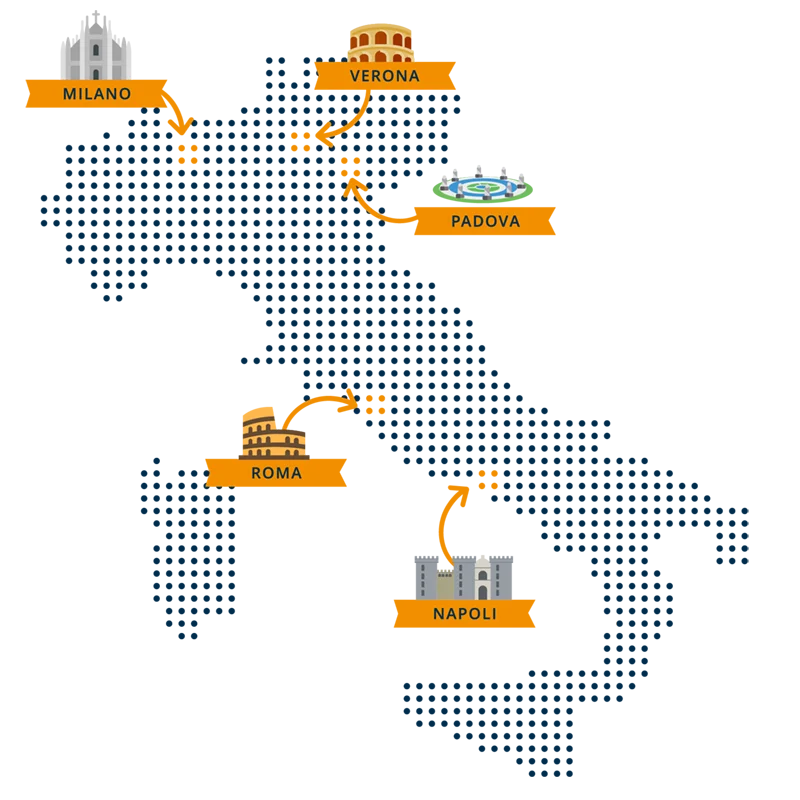
\includegraphics[width=0.45\textwidth]{images/sync_lab_sedi.png}
    \caption{Attuali sedi di Sync Lab}
    \captionsetup{aboveskip=2pt}
    \caption*{\begin{footnotesize}\textit{Fonte:} \url{https://www.synclab.it/}\end{footnotesize}}
  \end{center}
\end{figure}

Sync Lab ha fornito prodotti e consulenze a più di 150 clienti, distribuiti tra clienti diretti e finali, e attualmente possiede cinque sedi (figura \thefigure): Napoli, Roma, Milano, Padova e Verona.

L'azienda è suddivisa in molteplici settori dislocati nelle diverse sedi; l'esperienza personale mi ha portato a conoscere il settore dell'\textit{Enterprise Architecture Integration} e del \textit{Technical Professional Services Padova}.

\section{Servizi offerti dall'azienda}

Per comprendere appropriatamente il contesto che ha portato alla nascita del progetto di \stage\, è bene conoscere la tipologia di servizi e prodotti che l'azienda offre ai propri clienti.
Sync Lab offre per i propri clienti numerosi servizi, tra cui:
\begin{itemize}
  \item Valutazione e controllo progetti
    \begin{itemize}
      \item \textit{Planning e project management}; definizione di \textit{Milestone} e \textit{team} di progetto.
      \item Valutazione di impatto e \textit{risk analysis}; monitoraggio e \textit{benchmarking}.
      \item Valutazione e controllo di progetti \software\ attraverso l’utilizzo di metriche e modelli economici di stima e previsione.
    \end{itemize}
    \item Sistemi distribuiti di \textit{Enterprise}
      \begin{itemize}
        \item Progettazione e realizzazione di sistemi distribuiti \textit{Enterprise} in architettura \sacrfoot{j2ee}, \sacrfoot{ejb}, \sacrfoot{cobra} e \textit{Web Services}.
        \item Progettazione e realizzazione di sistemi basati su \sacrfoot{mom} e \sacrfoot{jms}.
      \end{itemize}
    \item Tecnologie \textit{\acrlong{oo}}
    \begin{itemize}
      \item Applicazione delle tecnologie \sacr{oo} all’analisi e progettazione di \software\ applicativo e di sistema e nella definizione di architetture distribuite \textit{enterprise}.
      \item Utilizzo di metodologie \sacr{oo} per progettazione di applicazioni e processi e \sacr{uml}, con supporto di strumenti di \textit{modeling}, applicazione e definizione di \textit{Design Pattern}.
    \end{itemize}
\end{itemize}
% \bigskip\noindent
% Esposizioni delle ragioni personali che hanno portato alla scelta di tale percorso.


\section{\textit{Way of working} aziendale}

% Esposizione delle norme organizzative (\textit{online meeting}, \textit{smart working}, presenze in sede), degli strumenti utilizzati nel rapporto con l’azienda (chat, email e \textit{Project Board}), e delle norme di progetto.
%
% \bigskip\noindent
% Processi interni in cui sono stato coinvolto: Sviluppo, Collaudo, Verifica, Formazione, Manutenzione/Evoluzione.

% \bigskip\noindent
% Breve presentazione dei ruoli delle persone coinvolte nel percorso di \textit{stage}.

\subsection{Processi interni}

Durante il percorso di \textit{stage} sono stato coinvolto nei processi aziendali di Formazione, Progettazione architetturale, Codifica, Verifica e Collaudo; i processi di Manutenzione ed Evoluzione sono stati solamente accennati in quanto al di fuori dello scopo del percorso.
Questi processi, nella mia esperienza personale, non sono delineati in modo rigido e rigoroso nei progetti di sperimentazione: ciò ha lo scopo di garantire libertà e flessibilità al team di sviluppo e di conseguenza all'intero progetto, attributi necessari in ambito sperimentale.

\begin{figure}[h]
  \begin{center}
    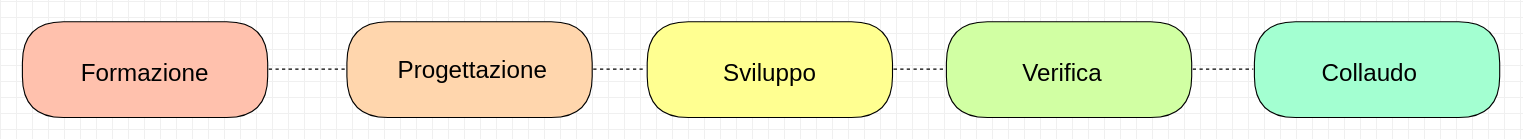
\includegraphics[width=\textwidth]{images/processi.png}
    \caption{Processi interni di cui ho avuto esperienza}
    \captionsetup{aboveskip=2pt}
    \caption*{\begin{footnotesize}\textit{Fonte: elaborazione personale}\end{footnotesize}}
  \end{center}
\end{figure}

Ogni processo è suddiviso in attività modulari, per rendere l'avanzamento efficace e quantificabile (in figura \thefigure\ sono illustrati i processi relativi allo \stage\, in ordine temporale da sinistra verso destra).

Per il processo di Formazione, Sync Lab fornisce materiale sotto forma di corsi \textit{online} tramite le piattaforme \textit{Coursera}\footfullcite{coursera} e \textit{Udemy}\footfullcite{udemy} e diapositive aziendali che illustrano i concetti chiave del settore \sacr{eai}.

Per il processo di Analisi, Sync Lab mi ha fornito il materiale relativo al caso d'uso da sviluppare, al fine di consentirmi la conoscenza dei requisiti e funzioni finali richieste dal prodotto.

Il processo di Progettazione architetturale è uno dei più complessi, che necessita di una buona dose di esperienza nell'ambito.
Per affrontare questo processo, oltre ad approfondire le mie conoscenze riguardo i diversi \textit{design pattern} e \textit{software architecture style}, l'azienda mi ha accompagnato e supportato nella progettazione stessa, con relative motivazioni.
Il tutor aziendale  Francesco Sanges e il responsabile del settore \sacr{eai} Salvatore Dore
sono stati di fondamentale aiuto in questo processo.

Il processo di Codifica nella mia esperienza personale è risultato abbastanza libero per quanto riguarda le tecnologie e i \software\ utilizzati, purché le scelte fossero adeguatamente motivate e adeguate.

Il processo di Verifica è stato eseguito dal tutor aziendale e dal Responsabile del settore \sacr{eai} a scadenza settimanale, tramite colloqui \textit{online} o resoconti sulla \textit{online board} di riferimento.

Il processo di Collaudo è avvenuto tramite una presentazione \textit{online} e dimostrazione \textit{live} del prodotto sviluppato all'intera azienda.

\subsection{Gestione di progetto}
% metodo piu appropriato per il team e per il progetto

% metodo agile

% L'azienda adotta dei processi interni per delineare l'avanzamento di un progetto.
Sync Lab utilizza una strategia di gestione di progetto (\textit{project management}) ispirata al metodo \textit{Agile}.

\noindent
La strategia \textit{Agile} è composta da quattro valori fondamentali:
\begin{itemize}
  \item gli individui hanno importanza maggiore rispetto ai processi;
  \item il funzionamento del \software\ ha la priorità rispetto alla documentazione esaustiva;
  \item la collaborazione tra fornitore e cliente è più importante della negoziazione del contratto;
  \item adattare il progetto ai cambiamenti ha la priorità rispetto al seguire la pianificazione.
\end{itemize}

Questo metodo di lavoro consente all'azienda un alto livello di adattabilità ed evoluzione del prodotto, in base alle richieste del cliente e alle esigenze del \textit{team} di progetto, al fine di fornire soluzioni \textit{ad-hoc} e soddisfare le loro richieste in modo efficiente ed efficace.

\subsection{Strumenti organizzativi}

Per mantenere un alto livello di organizzazione del progetto l'azienda fa uso di molteplici piattaforme dedicate al \textit{project management}, tra cui l'utilizzo di Kanban \textit{board} di progetto.
Questo tipo di \textit{board} sono specialmente adatte alla gestione di un progetto che utilizza la metodologia \textit{Agile} vista sopra.

\begin{figure}[h]
  \begin{center}
    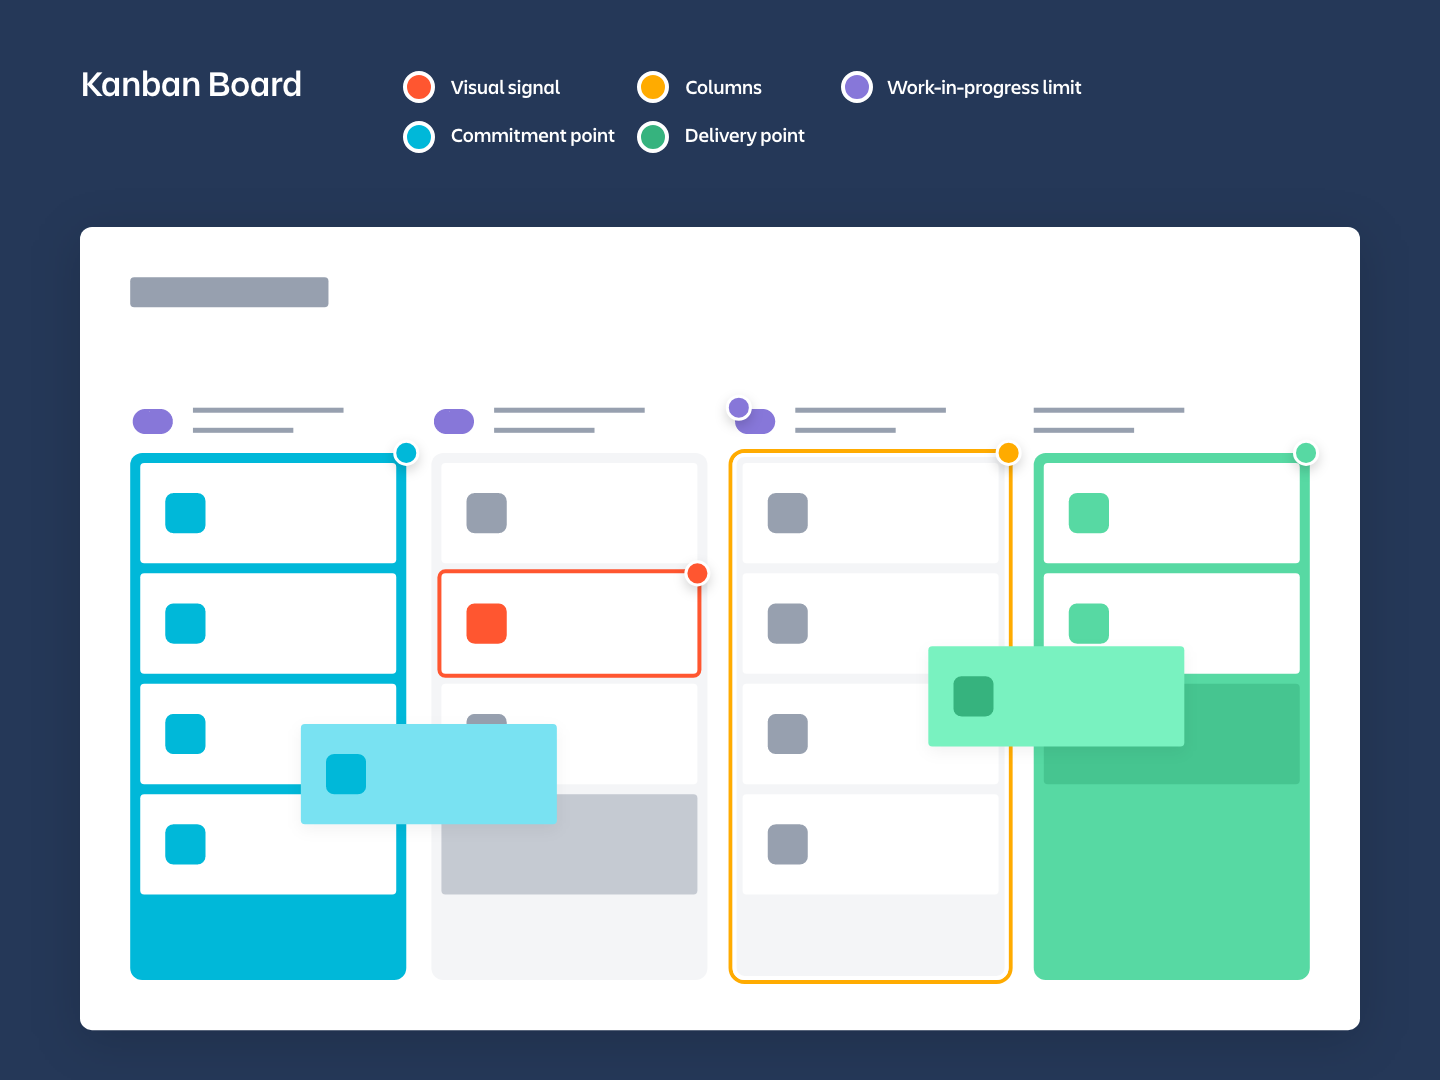
\includegraphics[width=\textwidth]{images/kanban.png}
    \caption{Schema riassuntivo degli elementi di una Kanban \textit{board}}
    \captionsetup{aboveskip=2pt}
    \caption*{\begin{footnotesize}\textit{Fonte:} \url{https://www.atlassian.com/agile/kanban/boards}\end{footnotesize}}
  \end{center}
\end{figure}

L'obiettivo di una Kanban \textit{board} è quello di presentare in modo rapido e chiaro una panoramica del progetto.
Lo stato di avanzamento delle attività è reso esplicito dalla posizione degli elementi, con un movimento che parte dall'estremo sinistro e si conclude all'estremo destro.

\noindent
Questo scopo viene raggiunto grazie al delineamento di cinque elementi principali:
\begin{itemize}
  \item delle \textit{card}, che contengono le diverse attività o \textit{ticket};
  \item delle colonne, che rappresentano lo stato d'avanzamento di ogni \textit{card};
  \item dei limiti di capacità imposti alle diverse colonne, con lo scopo di evitare impedimenti e rallentamenti nel flusso di lavoro;
  \item una colonna dedicata al \textit{commitment point} (punto di impegno), in cui vengono raccolte le varie idee o attività che possono essere implementate nel progetto;
  \item un punto di consegna (\textit{delivery point}), una colonna usualmente posta all'estremo destro della \textit{board}, che indica il completamento del lavoro richiesto per quell'attività.
\end{itemize}

Il percorso di \stage\ ha visto anch'esso l'utilizzo di una Kanban \textit{board} per la gestione del progetto.
\section{Dominio tecnologico}

% Sviluppo indipendente dal sistema operativo, produzione di \software\ non strettamente legati ad uno specifico linguaggio, utilizzo di ambienti virtuali quali \textit{Virtual Machine} e \textit{container} per simulare sistemi indipendenti.
% L'ambiente di lavoro di cui ho avuto esperienza risulta libero e flessibile, tanto nel campo organizzativo quanto in quello tecnologico.
\subsection{Un dominio flessibile e indipendente}

Il dominio tecnologico aziendale di cui ho avuto esperienza risulta libero e flessibile.

Lo sviluppo del prodotto \software\ nell'ambito del \sacr{eai} è fortemente consigliato essere indipendente dal linguaggio di programmazione, dagli strumenti utilizzati per l'esecuzione e sviluppo, e ove possibile e anche dal Sistema Operativo su cui esso esegue.
A tal scopo si utilizzano strumenti quali \textit{Virtual Machine} e \textit{Container}: essi non solo garantiscono l'indipendenza dal Sistema Operativo in uso, ma simulano efficacemente il caso d'uso reale in cui gli eseguibili sono dislocati in più dispositivi come spesso accade per il cliente finale.
Il percorso formativo ha visto l'apprendimento di entrambe le tecnologie tramite l'utilizzo dei \software\ \textit{Virtual Box}\footfullcite{virtualbox} e \textit{Docker}\footfullcite{docker}, ma infine solo quest'ultima è stata utilizzata durante il progetto.

Nonostante vi sia questa libertà tecnologica riguardo la scelta dei software e linguaggi, è necessario tenere in considerazioni i concetti principali vincolanti del settore, che descrivo in seguito.

 % come quelli di sistema distribuito, \sacrfoot{soa}, \textit{messaging pattern} e \sacrfoot{esb}.

\subsection{Sistemi distribuiti}

Un concetto fondamentale che caratterizza il dominio tecnologico aziendale, è quello del sistema distribuito, di cui l'azienda ha un forte interesse per soddisfare le necessità di integrazione dei suoi clienti.

\begin{figure}[h]
  \begin{center}
    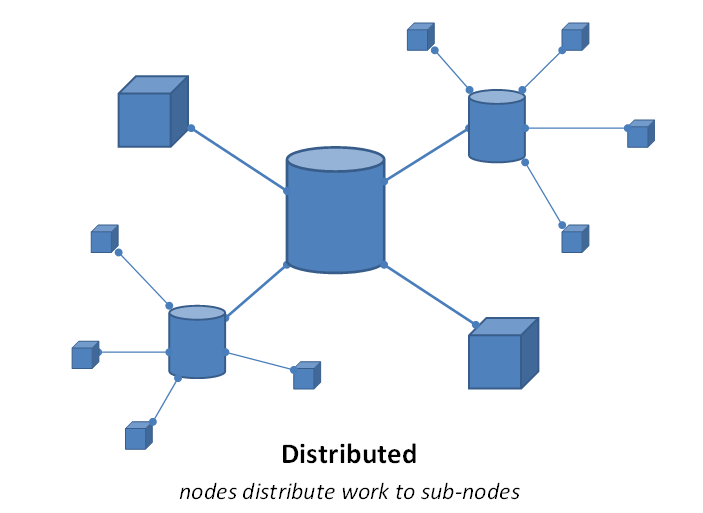
\includegraphics[width=0.45\textwidth]{images/distributed.png}
    \caption{Illustrazione di un sistema distribuito}
    \captionsetup{aboveskip=2pt}
    \caption*{\begin{footnotesize}\textit{Fonte:} \url{https://www.delphitools.info/DWSH/}\end{footnotesize}}
  \end{center}
\end{figure}

\textbf{Un sistema distribuito} (figura \thefigure) \textbf{è una collezione di componenti indipendenti} (spesso collocati in macchine differenti) \textbf{che condividono dei messaggi fra di loro per raggiungere un obiettivo comune.}
Un'architettura software basata su di un sistema distribuito necessita di una rete che connette tutti i singoli componenti (macchine, \textit{hardware} o \textit{software}), cosicché sia possibile lo scambio dei messaggi.

Il vantaggio principale di questo tipo di sistemi è la relativamente economica scalabilità orizzontale dei grandi sistemi: per migliorare la \textit{performance} del sistema è sufficiente aggiungere delle nuove macchine, meno costoso che richiedere \textit{hardware} sempre più potente.

Un secondo vantaggio di fondamentale importanza è la tolleranza ai guasti (\textit{fault tolerance}); rispetto ad un sistema centralizzato, ove nel caso di guasto nella macchina centrale si interrompe l'intero sistema, nel caso di un sistema distribuito esso continua a funzionare e fornire il servizio ove vi sia un guasto in un numero (limitato) di macchine.

Un ulteriore punto a favore dei sistemi distribuiti è la bassa latenza: il \textit{service client} si connette al nodo a se più geograficamente vicino, riducendo il tempo di risposta dei sistemi che coprono vasti territori.

Questo tipo di sistemi risulta molto favorevole per i clienti di grande dimensione di Sync Lab, per cui i vantaggi superano lo svantaggio del costo iniziale più alto dato dall'installazione del sistema.

\subsection{\textit{\acrlong{soa}}}

\begin{figure}[H]
  \begin{center}
    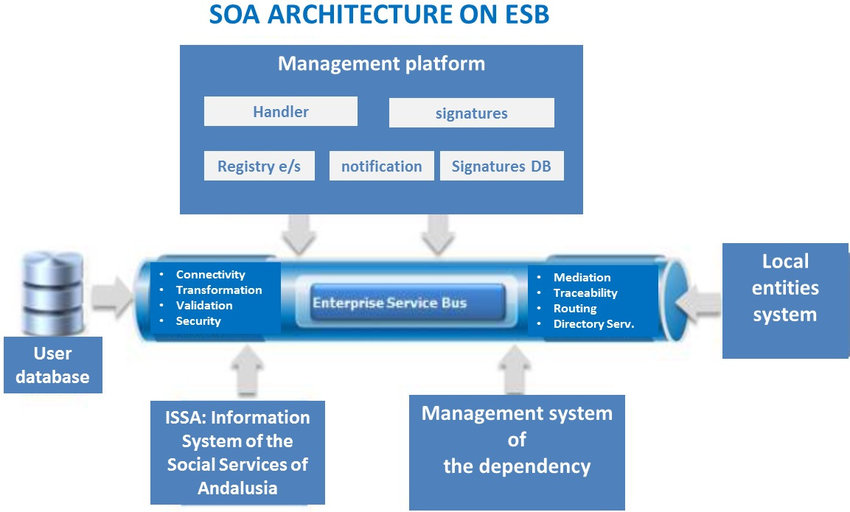
\includegraphics[width=0.75\textwidth]{images/soa_esb.jpg}
    \caption{\sacr{soa} applicata con un \sacr{esb}}
    \captionsetup{aboveskip=2pt}
    \caption*{\begin{footnotesize}\textit{Fonte:} \url{https://www.researchgate.net/figure/Fig-9-Service-Oriented-Architecture-SOA-Service-Oriented-Architecture-SOA-Service_fig7_330599363}\end{footnotesize}}
  \end{center}
\end{figure}

La \textit{\acrlong{soa}} è una tipologia di \textit{software architecture} spesso utilizzata in ambito \sacr{eai}.
Essa definisce un modo per rendere i componenti di un architettura \software\ riutilizzabili, tramite una decomposizione di un sistema in parti più piccole che comunicano tramite interfacce di servizio che possono essere classificate come sotto-sistemi.
\textbf{Ogni servizio in una \sacrfoot{soa} contiene il codice e le integrazioni dei dati necessari per eseguire una funzione aziendale completa e discreta}.
Le interfacce di servizio comportano un \textit{loose coupling}, il che significa che possono essere richiamate con poca o nessuna conoscenza della sottostante modalità di implementazione dell'integrazione.
I servizi sono esposti utilizzando protocolli di rete standard, come \sacrfoot{soap}/\sacr{http} o \sacrfoot{json}/\sacr{http}, per inviare richieste di lettura o modifica dei dati.
I servizi sono pubblicati per consentire agli sviluppatori di trovarli rapidamente e riutilizzarli per assemblare nuove applicazioni in modo modulare.

Questo tipo di architettura consente a Sync Lab di creare sistemi basati sui microservizi, derivati dalla \sacr{soa}, per dare modularità, scalabilità, flessibilità e facilità di manutenzione o aggiornamento ai propri prodotti.

\subsection{\textit{Messaging pattern}}

\begin{figure}[h]
  \begin{center}
    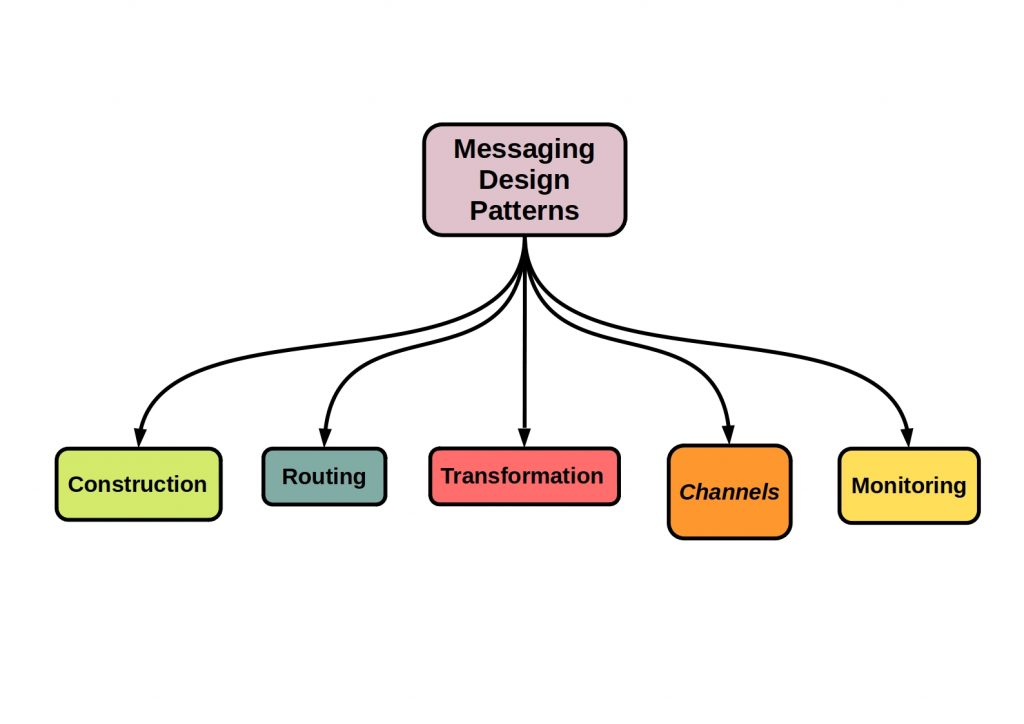
\includegraphics[width=0.65\textwidth]{images/messaging_pattern.jpeg}
    \caption{Schema di un \textit{messaging design pattern}}
    \captionsetup{aboveskip=2pt}
    \caption*{\begin{footnotesize}\textit{Fonte:} \url{https://starship-knowledge.com/messaging-patterns}\end{footnotesize}}
  \end{center}
\end{figure}

I \textit{messaging pattern} sono alla base di ogni sistema di integrazione.
Il \textit{design pattern} si occupa dello scambio di messaggi, come si può intuire dal nome.
Un messaggio è un pacchetto di dati atomico che può essere trasmesso attraverso un canale in modalità asincrona.
Un canale è un condotto virtuale che connette un servizio che invia i dati ad uno che li riceve.

Nella maggior parte dei sistemi di integrazione, il dato potrebbe necessitare diverse elaborazioni e non conoscere direttamente il destinatario del messaggio; è possibile applicare i concetti relativi alla \textit{pipes and filters architecture} inserendo un ricettore comune, un \textit{message router} che si occupa del \textit{routing} di tutti i messaggi e del passaggio di essi attraverso i vari filtri e trasformazioni.
Un \textit{message broker} è un modulo \software\ spesso posto all'interno di una \sacr{mom}; si occupa, oltre al \textit{routing}, della validazione, memorizzazione ed invio dei messaggi alle destinazioni appropriate


\subsection{\textit{\acrlong{esb}}}

\begin{figure}[H]
  \begin{center}
    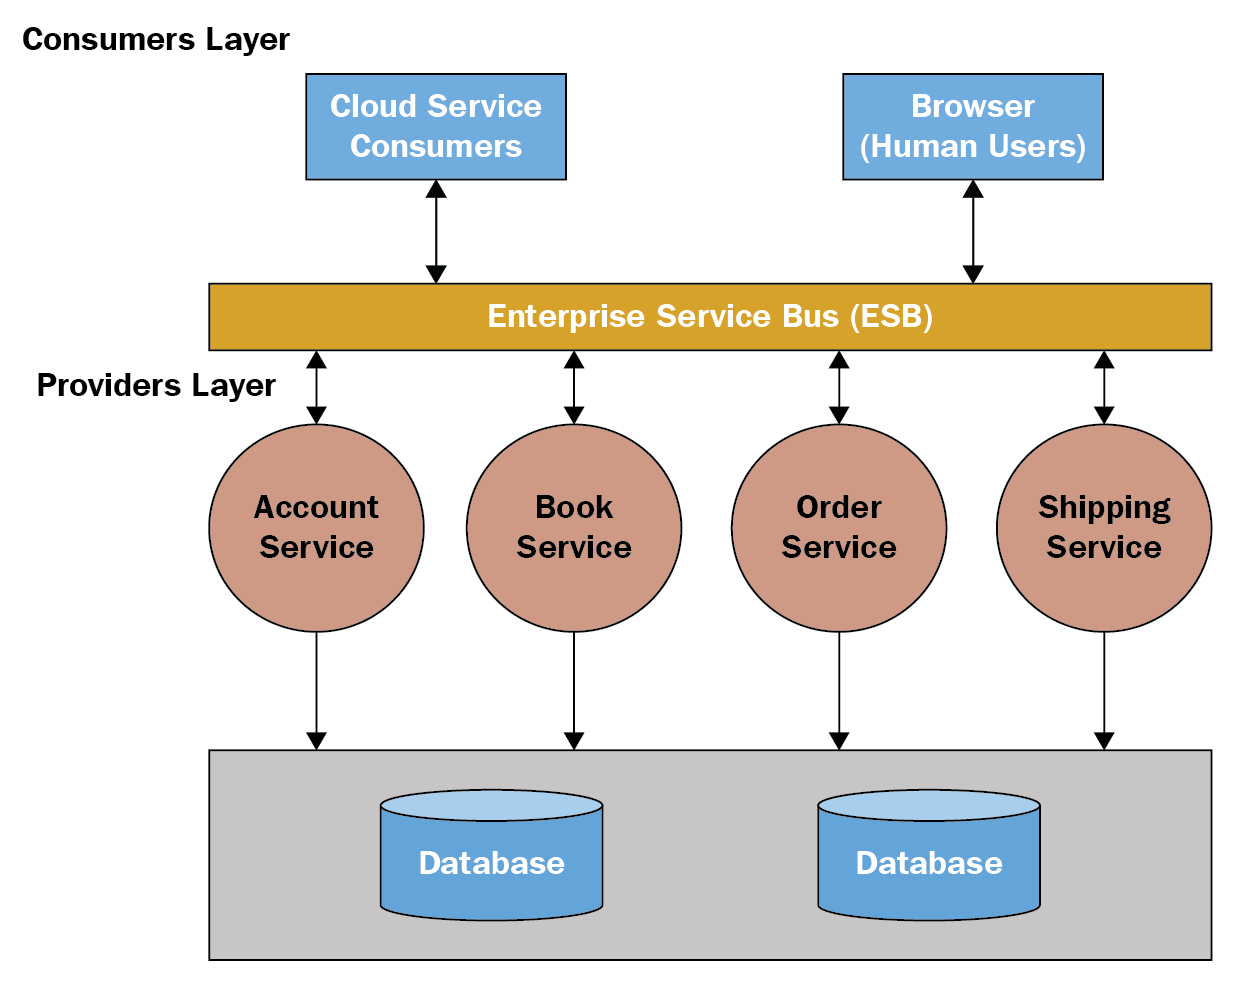
\includegraphics[width=0.65\textwidth]{images/esb.png}
    \caption{Illustrazione esemplificativa di un \sacr{esb}}
    \captionsetup{aboveskip=2pt}
    \caption*{\begin{footnotesize}\textit{Fonte:} \url{https://subscription.packtpub.com/book/application_development/9781789133608/1/ch01lvl1sec12/service-oriented-architecture-soa}\end{footnotesize}}
  \end{center}
\end{figure}

\textbf{Un \sacr{esb} è un \textit{pattern} architetturale in cui un \software\ centrale consente l'integrazione tra diverse applicazioni} (figura \thefigure).
Esso si occupa della comunicazione, trasformazione e conversione dei dati all'interno di una \sacr{soa}; è una tipologia più evoluta di \textit{message broker}.
Senza strumenti di questo tipo, la \textit{\acrlong{soa}} porterebbe ad un sistema composto semplicemente da un gruppo di servizi.
Ogni servizio dovrebbe occuparsi dello scambio di messaggi con tutti gli altri (\sacrfoot{p2p}) creando, nei sistemi più grandi, problemi per quanto riguarda l'estensione e manutenibilità dei servizi.

% \begin{figure}[h]
%   \begin{center}
%     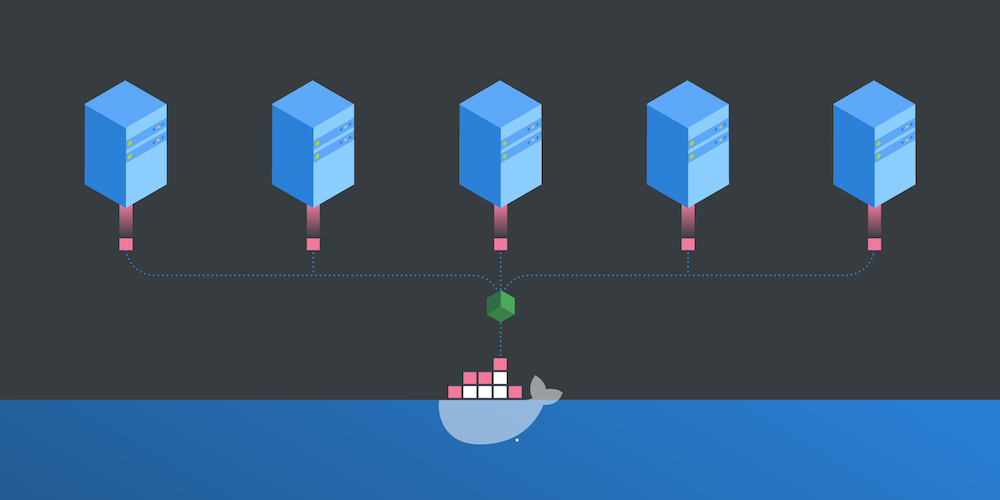
\includegraphics[width=0.75\textwidth]{images/docker_compose.png}
%     \caption{Illustrazione di un sistema a servizi indipendenti in container Docker}
%     \captionsetup{aboveskip=2pt}
%     \caption*{\begin{footnotesize}\textit{Fonte:} \url{https://pspdfkit.com/blog/2018/how-to-use-docker-compose-to-run-multiple-instances-of-a-service-in-development/}\end{footnotesize}}
%   \end{center}
% \end{figure}



% \section{Dominio applicativo}

\subsection{\sacr{eai} e \textit{Middleware}}

% L'esperienza di \textit{stage}
% Breve introduzione al settore del \textit{Enterprise Application Integration}, al tipo di clientela (ovvero pubblica e privata di grandi dimensioni, big data), alla tipologia di \software\ prodotti dall’azienda per la clientela (\textit{Middleware}), e alla propensione all’innovazione (richieste da parte della clientela
% In conclusione al percorso di studi del corso di laurea in Informatica ho effettuato lo \textit{stage} presso \textit{Sync Lab}.
% Sync Lab è un'azienda di produzione \software\ e integrazione di sistemi che fornisce principalmente prodotti a clienti di grande dimensione, sia pubblici che privati.
\begin{figure}[h]
  \begin{center}
    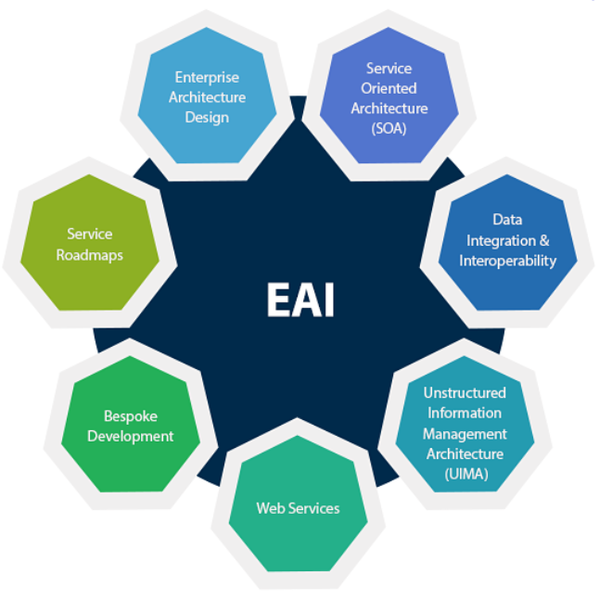
\includegraphics[width=0.48\textwidth]{images/eai.png}
    \caption{Concetti principali del \sacr{eai}}
    \captionsetup{aboveskip=2pt}
    \caption*{\begin{footnotesize}\textit{Fonte:} \url{https://commons.wikimedia.org/wiki/File:KrisangelChap2-EAI.png}\end{footnotesize}}
  \end{center}
\end{figure}

Il percorso di \textit{stage} intrapreso è associato al settore del \textit{Enterprise Architecture Integration}, che si occupa principalmente del \sacr{eai} (\textit{\acrlong{eai}}, figura \thefigure) ovvero dell'integrazione funzionale di applicazioni aziendali per una clientela di grandi dimensioni (come un'azienda di telecomunicazioni), tramite sistemi di integrazione e \textit{Middleware}.

I \textit{Middleware} e sistemi di integrazione prodotti comprendono l'utilizzo di molteplici linguaggi e tecnologie in continua evoluzione.\\
Dal sito di Red Hat\footfullcite{red-hat-middleware}:
% Dal sito di Red Hat\footnote{\textit{Cos'è il Middleware?}\url{https://www.redhat.com/it/topics/middleware/what-is-middleware}}:
\begin{displayquote}
  \textit{Il middleware è un software che fornisce alle applicazioni servizi e capacità frequentemente utilizzati, tra cui gestione dei dati e delle API, servizi per le applicazioni, messaggistica e autenticazione.\\
  Aiuta gli sviluppatori a creare le applicazioni in modo più efficiente e agisce come un tessuto connettivo tra applicazioni, dati e utenti.\\
  Può rendere conveniente lo sviluppo, l'esecuzione e la scalabilità di applicazioni alle organizzazioni con ambienti multi cloud e containerizzati.}
\end{displayquote}
\noindent
I \textit{Middleware} pertanto vedono due importanti utilizzi nel settore \sacr{eai}:
\begin{itemize}
  \item \textbf{Integrazione su più livelli:} i \textit{Middleware} connettono i principali sistemi aziendali interni ed esterni. Capacità di integrazione quali trasformazione, connettività, componibilità e messaggistica enterprise, abbinate all'autenticazione \sacrfoot{sso}, aiutano gli sviluppatori a estendere tali capacità su diverse applicazioni.
  \item \textbf{Flussi di dati:} le \sacrfoot{api} rappresentano una modalità per condividere i dati tra le applicazioni. Un altro approccio è quello del flusso di dati asincrono, che consiste nella replica di un set di dati in un livello intermedio, da cui i dati possono essere condivisi con più applicazioni.
  \item \textbf{Ottimizzazione di applicazioni esistenti:} con l'adozione del \textit{Middleware}, gli sviluppatori possono trasformare le applicazioni monolitiche esistenti in applicazioni \textit{cloud native} o a microservizi, mantenendo i validi strumenti già in uso ma migliorandone prestazioni e portabilità (figura \thefigure).
\end{itemize}

\begin{figure}[h]
  \begin{center}
    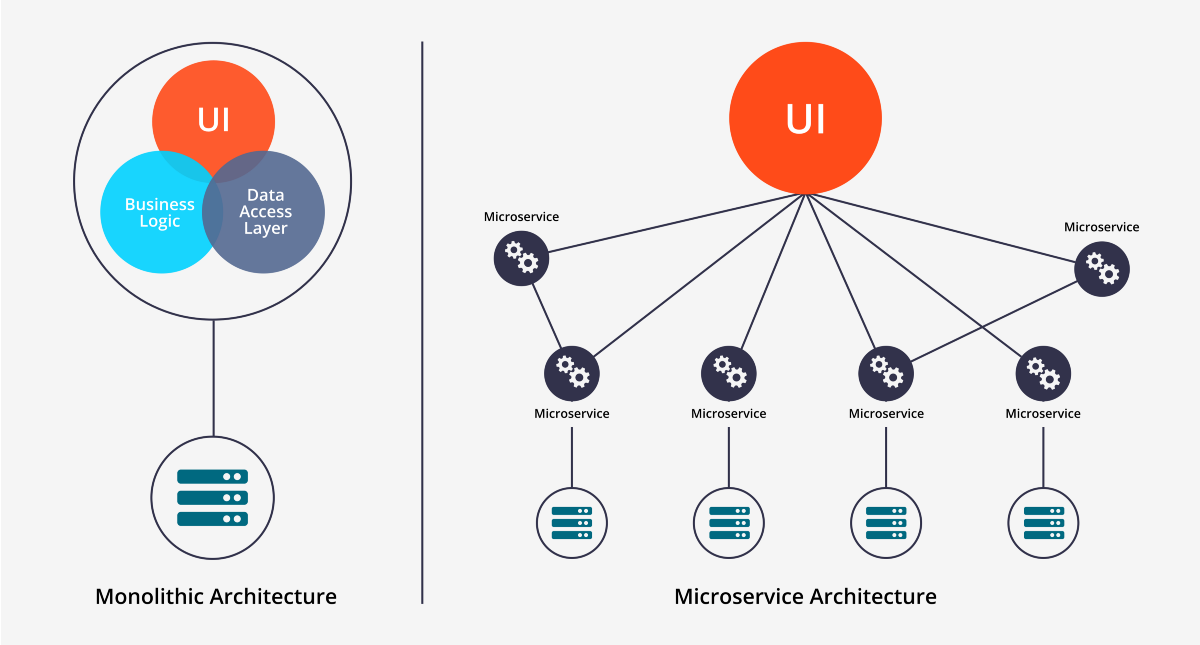
\includegraphics[width=0.85\textwidth]{images/mono_to_micro.png}
    \caption{Dalle classiche soluzioni monolitiche ai moderni sistemi a microservizi}
    \captionsetup{aboveskip=2pt}
    \caption*{\begin{footnotesize}\textit{Fonte:} \url{https://aymax.fr/en/why-a-microservices-architecture/}\end{footnotesize}}
  \end{center}
\end{figure}


\subsection{\textit{Container} e \textit{Virtual Machine}}

Come anticipato nella sezione precedente, tra le tecnologie più utilizzate in questo settore aziendale vi sono molte piattaforme che permettono di simulare ambienti distribuiti su più macchine fisiche, ove possibile anche indipendenti dal Sistema Operativo su cui viene eseguito il prodotto software.

La simulazione di questi \textit{distributed environment} avviene grazie a sistemi basati sul concetto di \textit{container} (come Docker e Kubernetes) oppure interi Sistemi Operativi che vengono eseguiti all'interno di una \textit{Virtual Machine}.
Il vantaggio principale di queste tecnologie è che rendono l'esecuzione del software al loro interno completamente indipendente dall'ambiente circostante, eliminando problemi di \sacrfoot{os} differenti tra i componenti del team o tra l'azienda e i clienti o divergenze nelle dipendenze con relative versioni.
Un \textit{container} o una \textit{Virtual Machine} contengono tutto il necessario affinché sia possibile eseguire il software al suo interno su diverse macchine fisiche (o anch'esse  virtuali).

Queste piattaforme non solo rendono agevole l'esecuzione del software prodotto, ma anche lo sviluppo: la condivisione, \textit{debugging} e manutenzione risultano più agevoli grazie alla condivisione dell'intero \textit{container} o \sacr{vm} con gli altri membri del team.

Inoltre, si adattano particolarmente bene a simulare l'ambiente distribuito, un concetto fondamentale nel settore del \textit{eai}; infatti è sufficiente generare molteplici \textit{container} o \sacr{vm} sulla stessa macchina fisica per simulare un sistema composto da più macchine fisiche distinte, minimizzando l'utilizzo di risorse senza compromettere il risultato del prodotto finale.
È così possibile per l'azienda riprodurre un sistema complesso che si avvicina alle risorse ed esigenze effettive del cliente, che usualmente possiede molti computer e server dislocati.

\begin{figure}[h]
  \begin{center}
    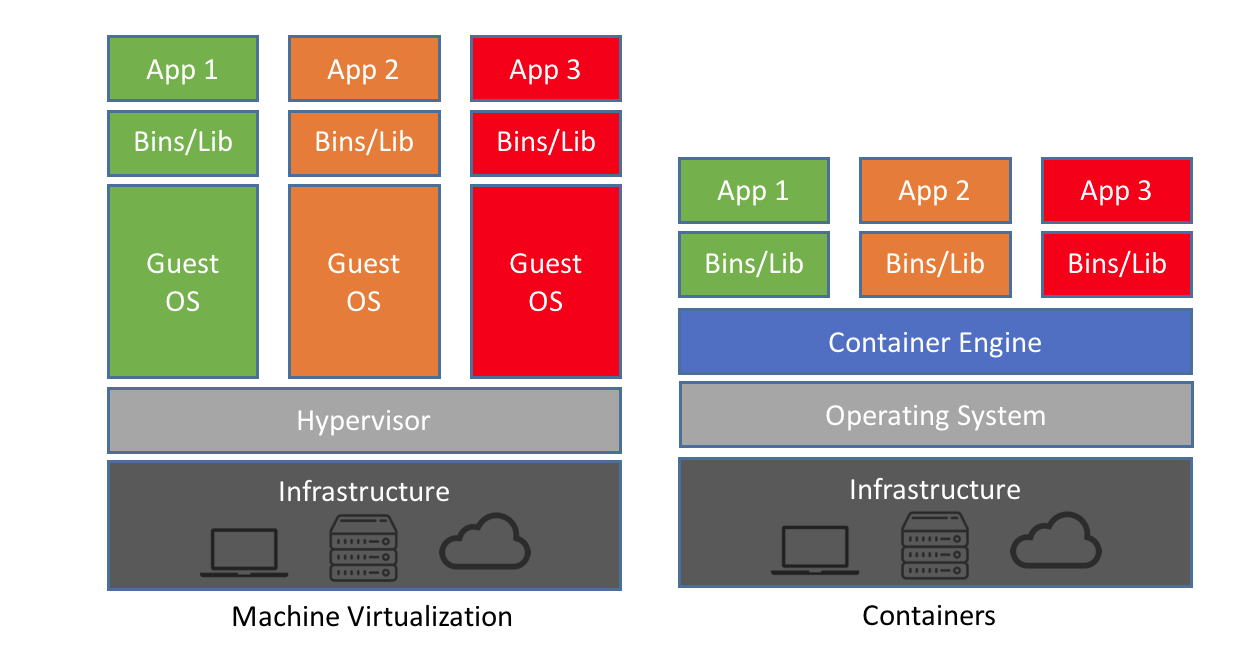
\includegraphics[width=0.85\textwidth]{images/vm_vs_container.png}
    \caption{Differenti implementazioni legate alle \sacr{vm} e \container}
    \captionsetup{aboveskip=2pt}
    \caption*{\begin{footnotesize}\textit{Fonte:} \url{https://pawseysc.github.io/container-workflows/01-docker-intro/index.html}\end{footnotesize}}
  \end{center}
\end{figure}

La figura \thefigure\ rappresenta graficamente le due diverse implementazioni delle due tecnologie.
Vi sono dunque delle notevoli differenze, vantaggi e svantaggi tra l'utilizzo dell'una e dell'altra, tra cui:
\begin{enumerate}
  \item i \container\ sono più rapidi delle \sacr{vm} nell'esecuzione;
  \item i \container\ sono più leggeri delle \sacr{vm} in termini di memoria;
  \item i \container\ sono più adatti a simulare un'architettura a microservizi, dato la relativa semplicità ed efficienza rispetto ad una \sacr{vm};
  \item le \sacr{vm} sono considerate tendenzialmente più sicure dei \container\;
  \item le infrastrutture e strumenti di gestione di grandi quantità di \sacr{vm} sono più consolidate dei corrispettivi strumenti associati ai \container.
\end{enumerate}

% Dati questi presupposti, ho optato per l'implementazione di un sistema basato su i \container\ nel mio progetto di \stage.
Durante il percorso di stage ho approfondito le mie conoscenze riguardo entrambe le tecnologie, optando di utilizzare i \container\ all'interno del mio progetto di \stage, poiché più efficiente considerate le risorse a mia disposizione.
La scelta della piattaforma di \container\ è stata quella di Docker.
% La scelta, in accordo con il tutor aziendale, è dovuta
Più precisamente, ho utilizzato l'estensione \textit{Docker-compose}\footfullcite{docker-compose} per gestire in modo elegante la generazione e collaudo di più servizi indipendenti (figura \thefigure): non solo questo \software\ consente di creare velocemente una rete di \textit{container} comunicanti su di una rete isolata, ma rende anche rapido ed efficiente lo sviluppo grazie alla possibilità di modificare e riavviare rapidamente un singolo servizio.
%
% \begin{figure}[H]
%   \begin{minted}[
%       xleftmargin=2em,
%       fontsize=\small,
%       bgcolor=lightgray!10,
%       autogobble=true,
%       numbers=left,
%       frame=none,
%       framesep=2mm,
%       baselinestretch=1]
%       {yaml}
%   version: "3.9"
%   services:
%     web:
%       build: .
%       ports:
%         - "5000:5000"
%       volumes:
%         - .:/code
%         - logvolume01:/var/log
%       links:
%         - redis
%     redis:
%       image: redis
%   \end{minted}
%   \caption{Frammento di codice che espone un esempio di ambiente \textit{multi-container} con docker-compose }
% \end{figure}
% \begin{mycode}{json}{Frammento di codice che espone un esempio di ambiente \textit{multi-container} con docker-compose}
%   version: "3.9"
%   services:
%     web:
%       build: .
%       ports:
%         - "5000:5000"
%       volumes:
%         - .:/code
%         - logvolume01:/var/log
%       links:
%         - redis
%     redis:
%       image: redis
% \end{mycode}

% \begin{mycode}{latex}{some caption}{code:label}
% My code here
% \end{mycode}
\begin{figure}[H]
  \begin{mycode}{yaml}
      version: "3.9"
      services:
        web:
          build: .
          ports:
            - "5000:5000"
          volumes:
            - .:/code
            - logvolume01:/var/log
          links:
            - redis
        redis:
          image: redis
  \end{mycode}
  \caption{Frammento di codice che espone un esempio di ambiente \textit{multi-container} con docker-compose}
  \captionsetup{aboveskip=2pt}
  \caption*{\begin{footnotesize}\textit{Fonte: elaborazione personale}\end{footnotesize}}

\end{figure}

Come si può vedere in figura \thefigure, è relativamente semplice e veloce creare un ambiente composto da due container (il servizio intitolato \texttt{web}, composto a partire dalla cartella corrente e accessibile alla porta 5000, e il servizio \texttt{redis}, generato a partire da un'immagine predefinita, entrambi connessi alla stessa rete locale di default di Docker.

Il caso d'uso realizzato nel mio percorso ha simulato grazie ai \container\ un sistema a microservizi che simula le risorse di un grande cliente gestore di telecomunicazioni, secondo una visione coerente con il tipo di clientela reale dell'azienda.
% TODO: completare il collegamento tra sopra e sotto;
% TODO: magari ci sta bene un esempio di dockerfile

\subsection{L'introduzione di Apache Kafka}

In questo periodo Sync Lab sta iniziando dei percorsi per implementare nuove tecnologie nei prodotti \textit{Middleware}.
Uno di questi prodotti è Apache Kafka.

Kafka è una piattaforma di \textit{event streaming}, un sistema distribuito e moderno basato sugli eventi anziché su di una soluzione più classica come può essere quella del \textit{request/response} e \sacr{p2p}.

L'\textit{event streaming} è una pratica focalizzata sul catturare dati in \textit{real-time} da diverse fonti come \textit{database}, sensori e dispositivi mobili sotto la forma di un flusso continuo di eventi; garantisce uno scambio continuo di informazioni e la loro interpretazione.

Apache Kafka è un \software\ fondato sul \textit{design pattern} del \textit{publish/subscribe}.
Contiene infatti delle \sacr{api} intitolate \textit{Producer} e \textit{Consumer}, che un utente della piattaforma può utilizzare rispettivamente per pubblicare degli eventi o riceverli istantaneamente.
Permette inoltre di memorizzare questo flusso di dati in modo affidabile, \textit{fault tolerant}, e duraturo, o di processare il flusso per processarlo e trasformarlo.

Un evento è definito come un'occorrenza significativa o un cambiamento di stato del sistema, e nell'ottica del \textit{messaging design pattern} occuperebbe il ruolo di un messaggio atomico.

\begin{figure}[H]
  \begin{center}
    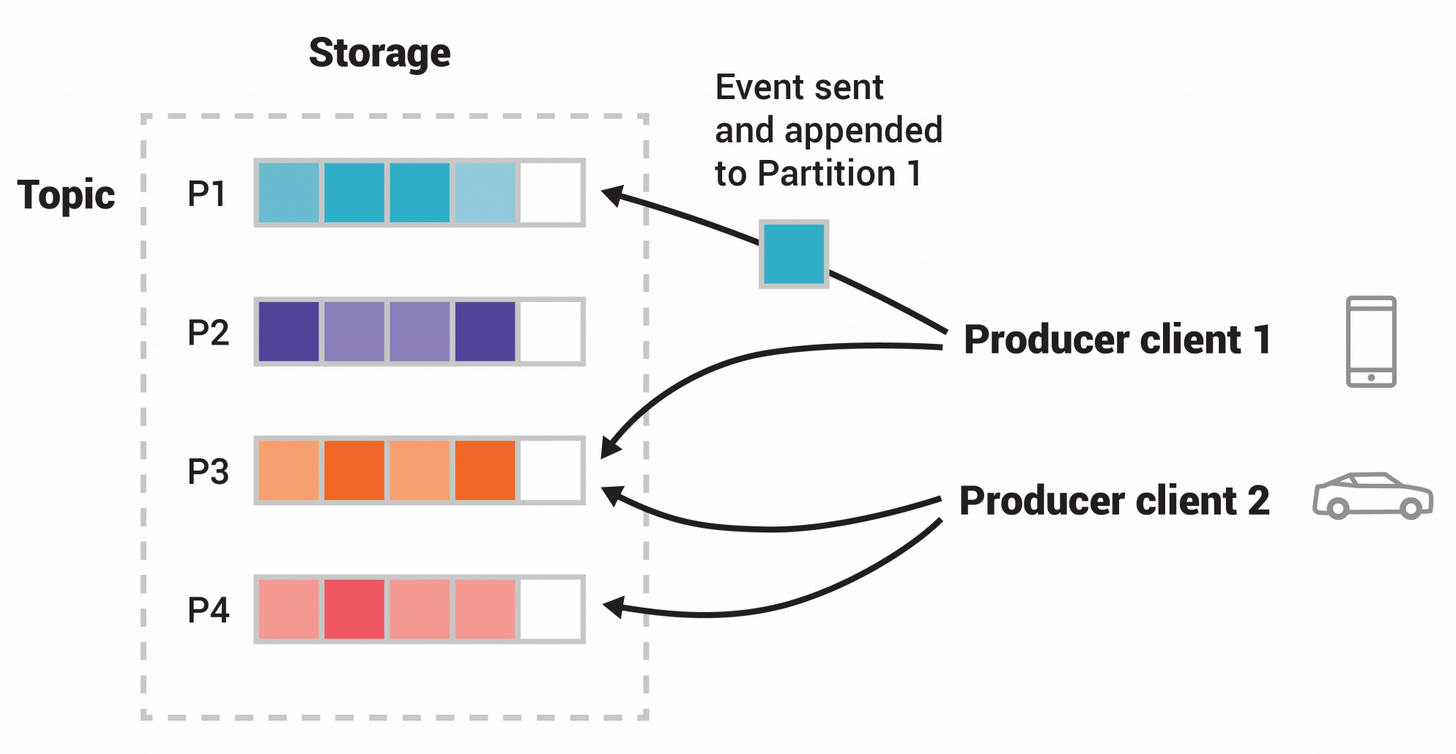
\includegraphics[width=0.85\textwidth]{images/topic.png}
    \caption{Schema di un topic contenente diversi eventi, diviso in partizioni (P), con molteplici \textit{producer}}
    \captionsetup{aboveskip=2pt}
    \caption*{\begin{footnotesize}\textit{Fonte:} \url{https://kafka.apache.org/intro}\end{footnotesize}}
  \end{center}
\end{figure}

Essi sono organizzati all'interno di \textit{topics}, delle liste ordinate di eventi in cui molteplici applicazioni possono scrivere o leggere tali eventi simultaneamente.
In figura si può vedere un esempio di \textit{topic}, diviso in diverse partizioni, in cui due \textit{producer} inseriscono dati simultaneamente.

Kafka viene eseguito come un gruppo (\textit{cluster}) di \textit{server} distribuiti.
Alcuni di questi \textit{server} sono chiamati \textit{broker}, e insieme compongono il livello di memorizzazione (\textit{storage layer}).
Altri \textit{server} sono dedicati all'esecuzione di Kafka Connect, un componente essenziale per l'importazione dei dati da altre fonti; esso è molto rilevante nel campo dei \middleware, poiché permette di integrare Kafka all'interno di sistemi pre-esistenti in modo graduale, con un investimento iniziale parziale.

I \textit{client} invece permettono di sviluppare applicazioni distribuite a microservizi che leggono, scrivono e processano il flusso di dati; questi \textit{client} mettono a disposizione delle interfacce per molti linguaggi e \software\ differenti, tra cui Java, Scala, Python, C++/C oltre a delle \sacr{rest} \sacr{api}.

Il sistema è molto adattabile, dato che può essere installato anche su \textit{acrlong{vm}}, \textit{container}, ambienti \textit{cloud} e addirittura \textit{bare-metal hardware}.
La piattaforma è costituita da un sistema distribuito di \textit{server} e \textit{client} che comunicano attraverso un protocollo \textit{network} \sacrfoot{tcp} ad alta \textit{performance}.

Il \software\ ha dimostrato negli anni recenti un notevole successo in diversi campi\footnote{Fonte: \url{https://kafka.apache.org/powered-by}}, come quello del flusso di \textit{Big Data}, del monitoraggio e dell'elaborazione dati in tempo reale.
L'adozione del \software\ nell'ambito del \sacr{eai} è in crescita dato le dimostrate qualità nel gestire grandi moli di dati: la sua performance, sicurezza e scalabilità sono i punti che hanno portato il software al suo attuale successo.

\section{L'innovazione all'interno dell'azienda}


Questo contesto dell'integrazione aziendale porta dunque l'impresa ad avere un'importante propensione all'innovazione, talvolta esplicitamente richiesta dai clienti.

Una direzione dell'evoluzione attuale nel settore \sacr{eai} riguarda la migrazione verso sistemi sempre più distribuiti, in accordo con l'ambiente di lavoro descritto nelle sezioni precedenti, in grado di gestire efficacemente ed in tempo reale flussi di dati in continua crescita e appartenenti al mondo del \textit{Big Data}.

L'avanguardia tecnologica è pertanto uno dei principali temi dell'azienda, che garantisce che essa rimanga sempre competitiva sul mercato dei sistemi di integrazione e nel settore dell'\sacr{eai}.
L'implementazione di nuove tecnologie, come può essere una \textit{\acrlong{eda}} basata su Kafka, permetterebbe a Sync Lab di offrire soluzioni sempre più moderne, scalabili e affidabili ai propri clienti.
